\chapter{Fundamentals}
\label{sec.fundamentals}

This chapter explains the basic terms and concepts that the thesis builds upon.
First, the programming language JavaScript is introduced and some of the most important properties of the language are highlighted as they are relevant for the implementations described in \autoref{sec.detection}.
Then, \hyperref[sec.browserAPIs]{browser APIs} and their functionality are described, followed by \hyperref[sec.browserExtensions]{browser extensions}.
Furthermore, the term \hyperref[sec.polyfill]{polyfill} is explained and an example of a polyfill showcased.
Finally, common browser security models and policies are introduced, starting with the \hyperref[sec.origin]{same-origin policy} and followed by the \hyperref[sec.csp]{\acf{csp}}.



\section{JavaScript}
\label{sec.javascript}

JavaScript is the predominant programming language used to build client-side web applications and browser extensions due to it being supported by all major browsers \cite{MozBrowserExtensionAPIs}. “Client-side” means that code is executed by the JavaScript engine of the browser, as opposed to code being executed by the server. There are many different JavaScript engines, the most notable ones being Google's V8 engine – which is most known for its use in Chromium \cite{V8}, Mozilla's SpiderMonkey used in Firefox \cite{SpiderMonkey} and Apple's JavaScriptCore used in Safari \cite{JavaScriptCore}.
Although the programming language was initially created as a scripting language for the web \cite{ECMA262_edition1}, it has since become a general purpose programing language and can also be used to build cross-platform applications for both desktop and mobile using frameworks such as Electron \cite{Electron} and React Native \cite{ReactNative}. It can even be used for sever-side applications with runtimes like Node.js, which is also powered by the V8 engine \cite{NodeJS}.

The name “JavaScript” is a trademark by Oracle, but the actual language the name refers to is called “ECMAScript”, which is a registered trademark of the nonprofit standards organization Ecma International and standardized by its TC39 committee. Ecma publishes specifications without using patents or, if necessary, only royalty-free patents and is also responsible for many other technological specifications, including the Office Open XML file formats and programming languages such as C\# and Dart \cite{EcmaStandards}. Ecma's TC39 committee includes all major browser vendors as part of its members, gathers bi-monthly for meetings and annually publishes new revisions (called “editions”) of the ECMAScript specification. The specification not only defines the language syntax, but also its semantics and libraries. \cite{TC39_general, TC39_activities}

JavaScript is an object-oriented programming language whose syntax was influenced by other programming languages such as C, Java, Self, and Scheme. Unlike the aforementioned languages however, JavaScript is not strict by default, allowing code to continue to execute even if certain syntactical and semantical errors are present. Current specifications of the language allow developers to change this behavior by activating the strict-mode with the statement \icode{"use strict";}, either for the entire script or single functions. In the strict-mode the language adds additional error conditions that need to be explicitly handled and restricts the use of certain features such as the \icode{with} statement. This can improve security and help developers uncover mistakes in their code. \cite{ECMA262_edition6}

The following subsections will highlight and explain key concepts of the language which will be relevant for \autoref{sec.browserAPIs} about browser APIs and later chapters such as \autoref{sec.detection} that will focus on the implementation of detection algorithms. First, \autoref{sec.scope} will define scopes and demonstrate their behavior in JavaScript, followed by an explanation of the global object in \autoref{sec.globals}. Finally, \autoref{sec.prototypes} introduces prototypes and the inheritance model of JavaScript objects.



\subsection{Scope}
\label{sec.scope}

The term “scope” refers to the context (or part of the code) in which variables are “visible“, meaning accessible. Variables that are accessible are generally also writable, except when explicitly declared otherwise, e.g. using the \icode{const} keyword. The top-level scope refers to the hierarchically highest scope of a script, which can either be the global scope or a module scope. JavaScript scopes can be categorized into the following four different types:

\begin{description}[font=\sffamily\bfseries, leftmargin=1cm, style=nextline]
\item[Global]
    Variables that are part of the global scope can be accessed from all scopes. Global variables can be declared using the \icode{var}, \icode{let} or \icode{const} keyword at the top-level. Additionally, in the non-strict mode, all expressions that assign a value to an unqualified identifier will result in the declaration of a new global variable. Variables declared using \icode{var} will also create a new property with the same name in the “global object”, which will be discussed separately in section \ref{sec.globals}. \cite{MozVar}

\item[Module]
    Modules, which allow splitting programs into separate files, pose an exception to the behavior described above. Each module has its own scope, and top-level declarations inside of modules are bound to the module scope instead of the global scope. \cite{MozVar}

\item[Function]
    Variable declarations inside of functions bind the variables to the function scope. \cite{MozVar}

\item[Block]
    A block is a group of statements which is delimited using a pair of braces (curly brackets). The \icode{var} keyword is not affected by block scopes and binds the declared variable to the next highest parent scope of the block scope that is either a function scope or the top-level scope \cite{MozVar}. Since the sixth edition of ECMAScript it is possible to bind variables to block scopes using the \icode{let} and \icode{const} keywords \cite{ECMA262_edition6}.
\end{description}

\begin{figure}[H]
    \centering
    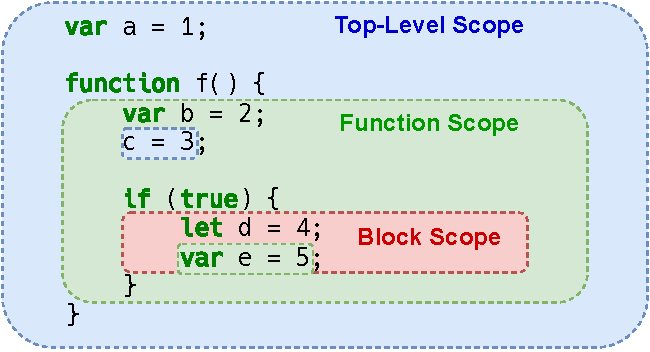
\includegraphics[width=9cm]{img/scope-4spaces.pdf}
    \caption{Scope of declared variables}
    \label{fig.scope}
\end{figure}

An example of variable declarations and the scope that they are bound to can be seen in \autoref{fig.scope}. Due to its definition in the top-level scope, the variable \icode{a} is bound to the global scope and visible to all scopes. In the function \icode{f}, the variable \icode{b} is bound to the function scope, while \icode{c} is part of the global scope, as it was not declared before the assignment. In the \icode{if} block, \icode{d} is part of the block scope due to the usage of \icode{let}, but \icode{e} is bound to the function scope, as \icode{var} does not bind variables to block scopes. Note that the function \icode{f} is also a global variable due to its definition in the top-level.



\subsection{Global Object}
\label{sec.globals}

The “global object” is an object that is always available in the global scope. Adding properties to the global object results in them also being accessible in the global scope. Global variables declared with \icode{var} and functions in the global scope are stored as properties of the global object, while variables created using \icode{let} and \icode{const} do not create such properties. The name of the global object varies depending on the context of where the code is executed. JavaScript code running in a web browser generally has a global object called \icode{window}, while web workers, which allow websites to execute JavaScript in the background and listen for notifications, use the global object \icode{WorkerGlobalScope} instead, and in Node.js the global object is simply called \icode{global}. \cite{MozGlobal}

The \icode{window} object represents the tab or window of the page running the code and provides an interface to various functions, including \hyperref[sec.browserAPIs]{browser APIs}. Its properties are generally isolated from other windows, with the exception of interfaces such as \icode{window.opener}, which are specifically designed to provide access to another window under certain conditions. \cite{MozWindow}



\subsection{Prototypes}
\label{sec.prototypes}

Similar to the typical class-based inheritance models of other object-oriented programming languages, JavaScript objects can inherit features from other objects via so-called prototypes. All JavaScript objects have a built-in property called prototype, which is an object itself and can also have a prototype, thereby creating a chain called the prototype chain. When accessing properties of an object, such as variables or methods, the property will first be looked for in the object itself. If the object does not contain a property, the prototype chain will be recursively traversed until either the desired property is found or \icode{null} – the end of the chain – is reached, in which case the resulting value will be \icode{undefined}. \cite{ECMA262_edition6, MozObjectPrototypes}



\subsection{Browser APIs}
\label{sec.browserAPIs}

Client-side web \acsp{api} are \acp{api} that are not built into the JavaScript language itself, but instead provided by the browser and its JavaScript engine. For the sake of clarity and readability this category of \acp{api} will be referred to as “browser \acsp{api}”.

Browser \acsp{api} consist of interfaces that allow scripts to interact with the page they are associated with, the browser, the device running the browser, device sensors and potentially also other connected devices. \acsp{api} not only expose additional features, but also act as an abstraction for the complexity associated with the implementation of commonly required functionalities to provide a simple interface for developers. \cite{MozWebAPIs}
One such interface is the \icode{document} object, which allows scripts to interact with the \ac{dom} and dynamically change the contents of \acs{html} documents through methods such as \icode{document.createElement()}, which creates a new element that can then be inserted into the page using methods such as \icode{document.body.append()} \cite{dom}. Another example is the fetch \acs{api}, which allows web applications to invoke network requests to dynamically send and receive data \cite{fetch}.

Furthermore, browser \acsp{api} also provide security related interfaces that handle sensitive data, such as the web authentication \acs{api} which allows web applications to implement secure authentication \cite{webauthn} or the web cryptography \acs{api} which provides secure implementations of common cryptographic algorithms that allow web applications to encrypt, decrypt, sign and verify data while abstracting the underlying implementations, secure key generation and management \cite{crypto}.

Browser APIs are globally accessible through the \hyperref[sec.globals]{global object} introduced in \autoref{sec.globals} and can generally be overwritten. The modification of browser \acsp{api} is not necessarily malicious, as it can be used to customize their behavior or, in the case of \hyperref[sec.polyfill]{polyfills}, to ensure the availability of certain \acsp{api} and provide consistent interfaces for web applications. This will be explained in more detail in \autoref{sec.polyfill}.



\section{Polyfills}
\label{sec.polyfill}

The term polyfill describes code that replicates the functionality of \acp{api} in environments that do not support them, such as outdated browsers. It usually refers to JavaScript code running in the browser that ensures the availability of certain \hyperref[sec.browserAPIs]{browser APIs} and that these \acsp{api} behave as defined by current or future specifications, regardless of the browser used to access the web application. In contrast to the term “shim”, polyfills provide a standardized interface for developers that acts as a “drop-in” replacement for the desired \acsp{api} instead of defining a new \acs{api}. \cite{MozPolyfill, RemyPolyfill}

Polyfills should only be used as a fallback, in case the required \acs{api} is not available or does not behave as expected, since their performance is not as good as that of native implementations and it is possible that they only support a subset of the full functionality. \cite{MozPolyfill}

As an example, we will take a look at how one would go about implementing a polyfill for the \icode{<String>.includes()} method, which can be called on strings to check if a string contains a given substring. This method was first specified in the 6th edition of ECMAScript published in 2015 \cite{ECMA262_edition6} and is therefore not implemented in old browsers such as Internet Explorer. Ideally, a polyfill should first check for the existence of a native implementation, which in this case can be achieved by evaluating \icode{String.prototype.includes}. If the function does exist in a browser, the aforementioned expression evaluates to true, meaning no polyfill is necessary. However, if it evaluates to false and thus does not exist, the code should add its own reimplementation of the includes function as a property of \icode{String.prototype}.

In the case of the \icode{<String>.includes()} method, a reimplementation of the native \acs{api} is trivial, as one can make use of the \icode{<String>.indexOf} method, which has been available since the first edition of ECMAScript published in 1997 \cite{ECMA262_edition1} and is therefore supported in all browsers. Aside from argument validation, the polyfill function only needs to call \icode{this.indexOf(search, start)}, which returns the position of a given substring in another string, and return \icode{true} if the position is $\ge 0$ and \icode{false} if the position is equal to $-1$, since the latter indicates that the string does not contain the given substring.



\section{Browser Extensions}
\label{sec.browserExtensions}

Browser extensions are a bundle of scripts and other resources that can add new functionality to a browser or change its behavior and \ac{ui} \cite{MozBrowserExtensions}. Browser extensions are generally written in JavaScript since all major browsers provide JavaScript \acsp{api} for extensions \cite{MozBrowserExtensionAPIs}. In addition to the \hyperref[sec.browserAPIs]{browser APIs} accessible to web pages, browser extensions have access to the browser extension \acsp{api}, which provide interfaces to control browser functionality such as bookmarks, tabs, notifications, browsing history, and are also able to intercept network requests and modify the content of web pages \cite{MozBrowserExtensions}.



\section{Origin and Same-Origin Policy}
\label{sec.origin}

Origins play an important role in the common security model used by browsers, known as the Same-Origin Policy. They are used to define which resources should be isolated from one another to prevent potentially malicious sites from accessing or interacting with third-party resources and reduce possible attack vectors. Pages of one origin usually only have limited or no access to resources that are part of a different origin. Data stored using the localStorage \acs{api} for example is only shared across the same origin, while cookies can also be shared across different origins \cite{html}. \cite{MozSameOriginPolicy}

The origin of a resource is determined by three parts of its \ac{uri}: scheme, domain and port. All resources with a matching triple of scheme, domain and port are part of the same origin. \cite{origin} The \acp{url} \icode{https://example.com/lorem} and \icode{https://example.com/ipsum} share the same origin, while \icode{http://example.com/lorem} and \icode{https://www.example.com/lorem} each have different origins, both from one another and from the first two \acp{url}, due to the difference in scheme and host respectively.



\section{Content Security Policy}
\label{sec.csp}

The \acf{csp} is a security feature that allows detecting and preventing the unintentional injection of resources into a web page by granularly declaring the sources where dynamic resources are allowed to be loaded from. It is intended to mitigate attacks such as \acf{xss} and monitor inclusions of untrusted resources in web applications. \cite{MozCSP}

To configure the policy, a web server needs to send the \icode{Content-Security-Policy} \acs{http} header with a valid policy configuration, or alternatively specify it using a \icode{<meta>} element in the \acs{html} document \cite{MozCSP}. For example, the following policy shown in listing \ref{lst.csp} could be used in order to block resources from everywhere except for the sites own origin, but allow images and other media to be loaded from the domain \icode{cdn.example.com}.

\begin{lstlisting}[language=CSP,numbers=none,label={lst.csp},caption={Example of a valid CSP policy}]
default-src 'self'; img-src cdn.example.com; media-src cdn.example.com
\end{lstlisting}

It is also possible to configure the \ac{csp} such that browsers send reports about violations of the policy to a desired endpoint using the \icode{report-uri} directive. The endpoint will receive reports in the form of \acs{json} encoded data. \cite{MozCSP}



\section{Browser Security Architecture}
\label{sec.browser-security-architecture}

This section explains the core concepts of the security architectures of browsers. It primarily focuses on the security architectures of Chromium and Firefox, which share similar approaches, but the concepts discussed here are also applicable to other browsers. Both Chromium and Firefox isolate the processing and rendering of web content from the rest of the browser and its \ac{ui}. Every web page has a separate rendering process, which is responsible for functionality such as parsing \acs{html}/\acs{css}, decoding images, interpreting JavaScript code, handling the \ac{dom} and rendering the page. Due to the complexity of the rendering engine and the fact that it needs to handle untrusted data from the web, these processes run in a sandbox that prevents them from directly accessing certain functionality of the \ac{os}. The sandbox is configured to have as few permissions as possible and prevents access to the filesystem – with a few exceptions such as temporary files that depend on the browser and \ac{os} – and also prevent access to the network. In order to send and receive data to/from the network, the rendering processes communicate with the main browser process using \ac{ipc}.~\cite{ChromiumSecArchitecture, MozFFSandbox}

\begin{figure}[H]
    \centering
    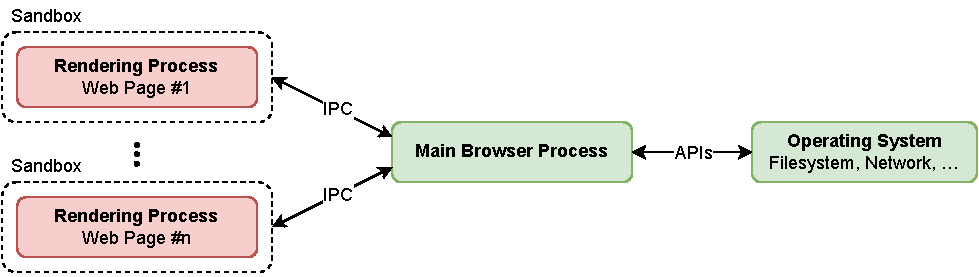
\includegraphics[width=16cm]{img/browser-process-model.pdf}
    \caption{Simplified Browser Process Model}
    \label{fig.browser-process-model}
\end{figure}

\autoref{fig.browser-process-model} depicts a simplified version of the actual process model, which also contains separate proccesses for \acs{gpu} rendering, browser extensions and more. The colors of the boxes represent the “trustworthyness”, with the red rendering process being considered untrusted due to its execution of potentially malicious code, while the green main browser process and \ac{os} are considered to be trusted. The sandbox allows the different trust environments to be isolated from each other and only interact through limited interfaces over \acs{ipc}. This means that even in a case where malicious web content manages to execute arbitrary code inside the rendering process through a security vulnerability, it would still not be able to access the filesystem, due to the restrictions of the sandbox. \cite{ChromiumSecArchitecture, MozFFSandbox}
